\chapter{Estado del arte} % Main chapter title

\label{chStateOfTheArt} % For referencing the chapter elsewhere, use \ref{Chapter1} 

%----------------------------------------------------------------------------------------


La Web contiene una gran cantidad de opiniones respecto a productos, políticos, y mucho mas, expresado en forma de noticias, sitios de opinión, reseñas en tiendas online, redes sociales. Como resultado, el problema de ``Minería de opinión'' ha obtenido una atención creciente en las ultimas dos décadas y es un factor decisivo para las nuevas organizaciones. De esto mismo partimos que el análisis de textos para extraer el significado y demás componentes extraíbles del texto componen un factor que debe considerarse al momento de realizar decisiones, de manera que los avances hechos hasta ahora tienen como meta una aplicación practica de lo que se conoce como \glsentrylong{nlp}.

Luego de los ataques terroristas del 11 de Septiembre de 2001 en Estados Unidos, se realizaron fuertes criticas respecto a la inteligencia, donde el director del FBI~\emph{Robert~S.~Mueller} indico que el principal problema que la agencia tuvo fue que se enfocaba demasiado en lidiar con el crimen luego de que fue cometido y ponía muy poco énfasis en prevenirlo. Es por esto que el uso de \gls{nlp} para temas de seguridad como también de metodologías de \glsentrylong{machinel} y \glsentrylong{deepl} han sido ampliamente utilizadas en ámbito de seguridad luego de estos eventos.

Para obtener una mejor inteligencia se necesito de mejores tecnologías a las que se tenían entonces (véase \cite[p\'ag 2]{mena2003investigative}):
\begin{itemize}
\item Integración de datos (\'o \gls{dataintegration} en ingl\'es)
\item Análisis de vínculos (\'o \gls{linkanalisys} en ingl\'es)
\item Agentes de software (\'o \gls{softwareagents} en ingl\'es)
\item Minería de texto (\'o \gls{textmining} en ingl\'es)
\item Redes neuronales (\'o \gls{neuralnetworks} en ingl\'es)
\item Algoritmos de \glsentrylong{machinel} (\'o \gls{mlalgorithms} en ingl\'es)
\end{itemize}

% ================================================================

\section{Análisis de vínculos (\glsentrylong{linkanalisys})}
Es la visualización de asociaciones entre entidades y eventos, por lo general involucran una visualización por medio de una gráfica o un mapa que muestre las relaciones entre sospechosos y ubicaciones, sea por medio físico o por comunicaciones en la red.

% ================================================================

\section{Agentes de software (\glsentrylong{softwareagents})}
Es el software que realiza tareas asignadas por el usuario de manera autónoma, donde sus habilidades básicas son:
\begin{itemize}
\item \textbf{Realización de tareas:} Hacen obtención de información, filtrado, monitoreo y reporte.
\item \textbf{Conocimiento:} Pueden usar reglas programadas, o pueden aprender reglas nuevas (véase \ref{secKBS}).
\item \textbf{Habilidades de comunicación:} Reportar a humanos e interactuar con otros agentes.
\end{itemize}

% ================================================================

\section{Sistemas Basados en Conocimiento (\glsentrylong{kbs})} \label{secKBS}
Según \cite{sajja2010knowledge}, los \gls{kbs} son uno de los mayores miembros de la familia de \gls{ai}.

\begin{figure}[th]
\centering
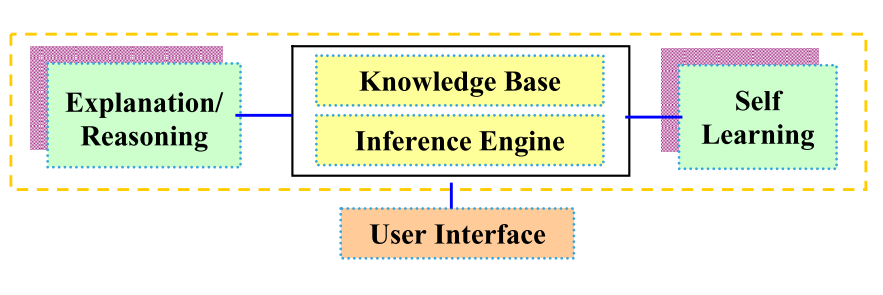
\includegraphics[scale=0.4]{Figures/kbs-architecture.png}
\decoRule
\caption[Arquitectura \gls{kbs}]{Arquitectura \gls{kbs}. Tomado de \cite{sajja2010knowledge}}
\label{fig:kbs-arch}
\end{figure}

\subsection{Fuzzy Knowledge Based Systems}
Pendiente

% ================================================================

\section{Mineria de texto (\glsentrylong{textmining})} \label{secNLP}
Es un subcampo de Inteligencia Artificial conocida como \glsentrylong{nlp}, en donde las herramientas de minería de datos pueden capturar rasgos críticos del contenido de un documento basado en el análisis de sus características lingüísticas.

La mayoría de los crímenes son electrónicos por naturaleza, por lo que se dejan rastros textuales que investigadores pueden seguir y analizar.Estas se enfocan en el descubrimiento de relaciones en texto no--estructurado y pueden ser aplicados al problema de \emph{búsqueda} y \emph{localizar palabras clave}.

% ================================================================

\section{Redes Neuronales (\glsentrylong{neuralnetworks})} \label{secNN}
Pendiente

\subsection{Sistemas de Detección de Anomalías (\glsentrylong{anomalydetectionsys})}
Pendiente

\subsection{Mapa autoorganizado (\glsentrylong{som})}
Pendiente
\begin{figure}[th]
\centering
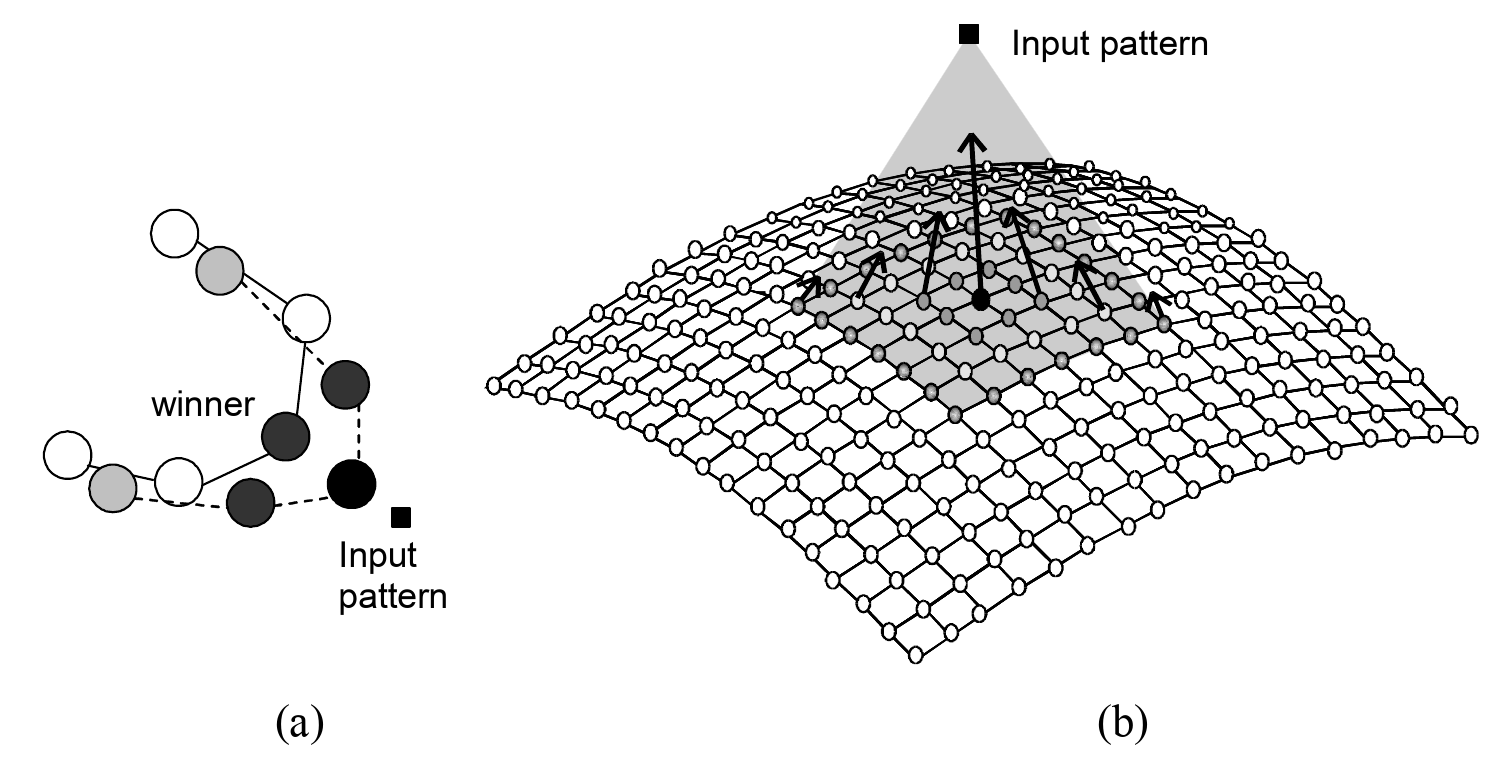
\includegraphics[scale=0.2]{Figures/som-adaptive-proc.png}
\decoRule
\caption[Proceso de adaptación de \gls{som}]{Proceso de adaptación de \gls{som}. Tomado de \cite{de2006fundamentals}}
\label{fig:som-adap-proc}
\end{figure}

\begin{figure}[th]
\centering
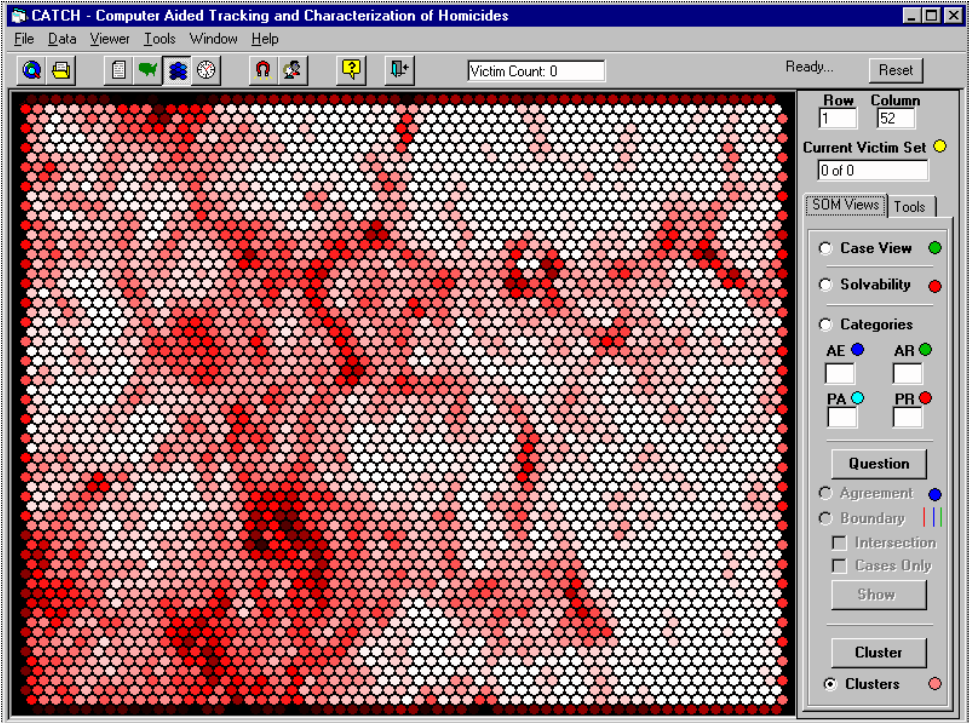
\includegraphics[scale=0.3]{Figures/som-example.png}
\decoRule
\caption[Ejemplo de uso de \gls{som}]{Ejemplo de uso de \gls{som}. Tomado de \cite{mena2003investigative}}
\label{fig:som-example}
\end{figure}

% ================================================================

\section{Aprendizaje de maquina (\glsentrylong{machinel})} \label{secML}
Pendiente